\chapter{State of the Art}


\section*{Introduction}
We will introduce in this chapter some useful definitions and concepts that she
light on  the project. We will also assess the current situation be examining
the literature as well as the current solutions adopted by Predictix. Next, we
will specify the different proposed solutions and choose the one that fits most
our needs.
\pagebreak

\section{General concepts}

In this section, we will be defining the general concepts that the Technical
Infrastructure team work around, and more specifically those that this project
evolves around. We will also clarify the use cases for these technologies and
concepts in Predictix.

\section{Declarative programming}
In computer science, declarative programming is a programming paradigm—a style
of building the structure and elements of computer programs—that expresses the
logic of a computation without describing its control flow.[1]

Many languages that apply this style attempt to minimize or eliminate side
effects by describing what the program must accomplish in terms of the problem
domain, rather than describe how to accomplish it as a sequence of the
programming language primitives[2] (the how being left up to the language's
implementation). This is in contrast with imperative programming, which
implements algorithms in explicit steps.

Declarative programming often considers programs as theories of a formal logic,
and computations as deductions in that logic space. Declarative programming may
greatly simplify writing parallel programs.[3]

\subsection{Datalog}
Datalog is a declarative logic programming language that syntactically is a
subset of Prolog. It is often used as a query language for deductive databases.
In recent years, Datalog has found new application in data integration,
information extraction, networking, program analysis, security, and cloud
computing.

Its origins date back to the beginning of logic programming, but it became
prominent as a separate area around 1977 when Hervé Gallaire and Jack Minker
organized a workshop on logic and databases.[2] David Maier is credited with
coining the term Datalog.

The applications that we will measure the perforamnce of, are all written in
commercial implementation of Datalog, LogiQL.

\section{REST architecture}
Rest stands fore REpresntational State Transfer. It is an architecture style for
designing networked applications. It permits creating, modifying resources
easily. Indeed REST is a lightweight alternative to complex mechanism like RPC,
CORBA and SOAP. 

Rest is not a 'standard'. In fact,  it is a guideline to build an efficient
framework for communication between two machines using HTTP protocol. The World
Wide Web itself, based on HTTP, can be viewed as a REST-based architecture. REST
relies on a stateless, client-server, cacheable communication protocol. It is
simple to implement and maintain. In addition, it allows applications to be scalable
by supporting multiple backend services at the same time.

Much like Web Services, a REST service is platform-independent,
language-independent standard-based asit runs on top of HTTP, and is easily used
in the presence of firewalls.

However, there are a few major concepts which make REST unnique from other web
services. In fact , its main key principales are the following:

$\bullet$ \textbf{Unique URL-Resource mapping}: Every resouce is mapped to a unique URL. That
refers to a some logical way  to access information. 

$\bullet$ \textbf{Statelessness}: All information required to precess the request by server is
contained along with the request. This means that no informatio of the previes
request is maintained by the server. This is inherited from the fact that REST
is based on HTTP.

$\bullet$ \textbf{Action Verbs}: REST architecture use HTTP verbs to identify the apropriate
action. The main HTTP verbs used in a REST architecture are GET, POST, PUT and
DELETE. In fact, GET is used by the client to access the resource on the server,
PUT to update a resource, POST to create a new one and DELETE to remove
resource.

$\bullet$ \textbf{Data Exchange formats}: REST architecture does not require any particular
encoding for the resource body. JSON and XML are the most used format, but it
can be PROTOBUF, YAML etc. 

\section{Cloud}

Cloud computing is a type of Internet-based computing that provides shared
computer processing resources and data to computers and other devices on demand.
It is a model for enabling ubiquitous, on-demand access to a shared pool of
configurable computing resources (e.g., computer networks, servers, storage,
applications and services), which can be rapidly provisioned and released
with minimal management effort. Cloud computing and storage solutions provide
users and enterprises with various capabilities to store and process their data
in either privately owned, or third-party data centers that may be located
far from the user–ranging in distance from across a city to across the world.
Cloud computing relies on sharing of resources to achieve coherence and economy
of scale, similar to a utility (like the electricity grid) over an electricity
network.

\section{Retail}
TODO

\section{SaaS}
Software as a service (SaaS) is a software licensing and
delivery model in which software is licensed on a subscription basis and is
centrally hosted. It is sometimes referred to as "on-demand software",
and was formerly referred to as "software plus services" by Microsoft. SaaS
is typically accessed by users using a thin client via a web browser. SaaS has
become a common delivery model for many business applications, including office
and messaging software, payroll processing software, DBMS software, management
software, CAD software, development software, gamification, virtualization,[4]
accounting, collaboration, customer relationship management (CRM), Management
Information Systems (MIS), enterprise resource planning (ERP), invoicing, human
resource management (HRM), talent acquisition, content management (CM), and
service desk management. SaaS has been incorporated into the strategy of
nearly all leading enterprise software companies.

\section{Automation}
Automation or automatic control, is the use of various control systems for
operating equipment such as machinery, processes in factories, boilers and heat
treating ovens, switching on telephone networks, steering and stabilization of
ships, aircraft and other applications and vehicles with minimal or reduced
human intervention. Some processes have been completely automated.

Automation has been achieved by various means including mechanical, hydraulic,
pneumatic, electrical, electronic devices and computers, usually in combination.
Complicated systems, such as modern factories, airplanes and ships typically use
all these combined techniques. The biggest benefit of automation is that it
saves labor; however, it is also used to save energy and materials and to
improve quality, accuracy and precision.

The term automation in the software industry has gain a lot of success in the
recent years. From the automation of build to the deployment, various steps
in the develompent pipeline can be automated. Including benchmarking the
applications.

\section{Benchmark}
In computing, a benchmark is the act of running a computer program, a set of
programs, or other operations, in order to assess the relative performance of an
object, normally by running a number of standard tests and trials against it.[1]
The term 'benchmark' is also mostly utilized for the purposes of elaborately
designed benchmarking programs themselves.

Benchmarking is usually associated with assessing performance characteristics of
computer hardware, for example, the floating point operation performance of a
CPU, but there are circumstances when the technique is also applicable to
software. Software benchmarks are, for example, run against compilers or
database management systems.

Benchmarks provide a method of comparing the performance of various subsystems
across different chip/system architectures.

In our case the we are going to benchmark applications along with the database
system that powers them. Since they are strongly coupled.

\section{NoSQL}
A NoSQL (originally referring to "non SQL", "non relational" or "not only
SQL") database provides a mechanism for storage and retrieval of data which
is modeled in means other than the tabular relations used in relational
databases. Such databases have existed since the late 1960s, but did not obtain
the "NoSQL" moniker until a surge of popularity in the early twenty-first
century, triggered by the needs of Web 2.0 companies such as Facebook,
Google, and Amazon.com. NoSQL databases are increasingly used in big
data and real-time web applications.[6] NoSQL systems are also sometimes called
"Not only SQL" to emphasize that they may support SQL-like query
languages.

Motivations for this approach include: simplicity of design, simpler
"horizontal" scaling to clusters of machines (which is a problem for relational
databases), and finer control over availability. The data structures used by
NoSQL databases (e.g. key-value, wide column, graph, or document) are different
from those used by default in relational databases, making some operations
faster in NoSQL. The particular suitability of a given NoSQL database depends on
the problem it must solve. Sometimes the data structures used by NoSQL databases
are also viewed as "more flexible" than relational database tables

\section{SOA}
Service-Oriented Architecture(SOA) is primarily regarded as a technical
architecture consisting of tools and service specification to build loosely
coupled applications. At another level it is also a means to leverage
flexibility and agility to system services as it offers a hierarchical framework
to coordinate simultaneous business process design and implementations using
loosely coupled service infrastructures. SOA has been debated both in the
academy and industry and misinterpretations of its nature impede its adoption.
Web service is the most popular technical architecture applied in SOA, among
which the most popular and commercially successful platform is SOAP messaging
protocol. In SOAP Web service invocations must be carried that are compliant to
SOAP messaging standard. Services are described in a service description
standard called WSDL. Since SOAP allows multiple message exchange patterns such
as request-and-response, broadcasting and sophisticated message correlations, it
can be used to integrate almost all kinds of legacy system from different
vendors.
TODO(http://aisel.aisnet.org/cgi/viewcontent.cgi?article=3331&context=cais)

Basic technologies such as (XML, SOAP, WSDL) provide means to describe, locate,
and invoke services in SOA as an entity in its own right. However, these technologies
do not give a rich behavioral detail about the role of the service in more
complex collaboration. This collaboration includes a sequence of activities and
relationships between activities, which build the business process. There are
two ways to build this process: service orchestration and service choreography.

\subsection{Service orchestration}

Service orchestration represents a single centralized executable business
process (the orchestrator) that coordinates the interaction among different
services. The orchestrator is responsible for invoking and combining the
services.

\begin{figure}[h]
  \centering
  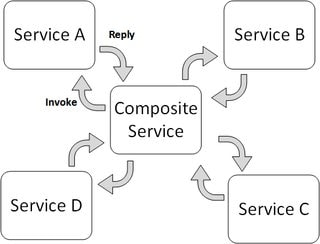
\includegraphics[width=7cm]{orch.jpg}
  \caption{Service orchestration}
\label{fig:orch}
\end{figure}

The relationship between all the participating services are described by a
single endpoint (i.e., the composite service). The orchestration includes the
management of transactions between individual services. Orchestration employs a
centralized approach for service composition.

\subsection{Service Choreography}

Service choreography is a global description of the participating services,
which is defined by exchange of messages, rules of interaction and agreements
between two or more endpoints. Choreography employs a decentralized approach for
service composition.

\begin{figure}[h]
  \centering
  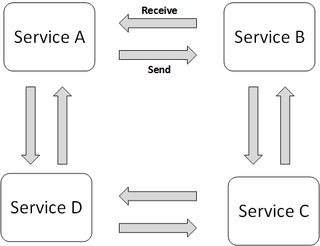
\includegraphics[width=7cm]{chor}
  \caption{Service choregraphy}
\label{fig:chor}
\end{figure}

The choreography describes the interactions between multiple services, where as
orchestration represents control from one party's perspective. This means that a
choreography differs from an orchestration with respect to where the logic that
controls the interactions between the services involved should reside.

\section{BPMN}
The Business Process Management Initiative (BPMI) has developed a standard
Business Process Modeling Notation (BPMN). The BPMN 1.0 specification was
released to the public in May 2004. This specification represents more than two
years of effort by the BPMI Notation Working Group. The primary goal of the BPMN
effort was to provide a notation that is readily understandable by all business
users, from the business analysts who create the initial drafts of the
processes, to the technical developers responsible for implementing the
technology that will perform those processes, and, finally, to the business
people who will manage and monitor those processes. BPMN will also be supported
with an internal model that will enable the generation of executable BPEL4WS.
Thus, BPMN creates a standardized bridge for the gap between the business
process design and process implementation.
BPMN defines a Business Process Diagram (BPD), which is based on a flowcharting
technique tailored for creating graphical models of business process operations.
A Business Process Model, then, is a network of graphical objects, which are
activities (i.e., work) and the flow controls that define their order of
performance.


\section{Agile}
The Agile Method is a particular approach to project management that is utilized
in software development. This method assists teams in responding to the
unpredictability of constructing software. It uses incremental, iterative work
sequences that are commonly known as sprints. Were a sprint is a period of time
allocated for a particular phase of a project. Sprints are considered to be
complete when the time period expires. There may be disagreements among the
members of the team as to whether or not the development is satisfactory;
however, there will be no more work on that particular phase of the project. The
remaining phases of the project will continue to develop within their respective
time frames.
\subsection{Scrum}
Scrum is just one of the many iterative and incremental agile software
development method. In the SCRUM methodology a sprint is the basic unit of
development. Each sprint starts with a planning meeting, where the tasks for the
sprint are identified and an estimated commitment for the sprint goal is made. A
Sprint ends with a review or retrospective meeting where the progress is
reviewed and lessons for the next sprint are identified. During each sprint, the
team creates finished portions of a product.

\section*{Conclusion}
TODO
